\chapter[Avaliação de Capacidade]{Avaliação de Capacidade}
% ----------------------------------------------------------
Dadas as definições e formalizações propostas no anteriormente, faz-se necessária
a especificação de uma lógica de manipulação das entidades e operações descritas.

Passamos agora a descrever uma proposta de processo de de avaliação de capacidade
a fim de buscar as Configurações de menor preço capazes de executar uma determinada 
Carga de Trabalho. Esse processo foi implementado como parte de um sistema 
computacional ao qual demos o nome de \textit{Cloud Capacitor}.  

Cloud Capacitor é um arcabouço para implementação de sistemas de avaliação de 
capacidade em ambientes de nuvem de infraestrutura como serviço. Ele permite que 
sejam implementadas lógicas customizadas de avaliação do desempenho resultante
da execução da Aplicação sob Teste. Essas lógicas são então reconhecidas pelo Cloud 
Capacitor como Estratégias de Avaliação.

As Estratégias devem implementar um conjunto de operações pré-definidas no processo 
que as torna capazes de se comunicar com o processo de avaliação de capacidade. Tais 
operações dão suporte ao processo nos momentos em que devem ser analisados os dados
dos resultados das execuções da Aplicação. Diferentes estratégias podem tomar 
decisões diferentes a partir dos mesmos dados de resultado.

\begin{figure}[htb]
  \caption{\label{fig_arq_alto_nivel}Arquitetura de alto nível do Cloud Capacitor}
  \begin{center}
    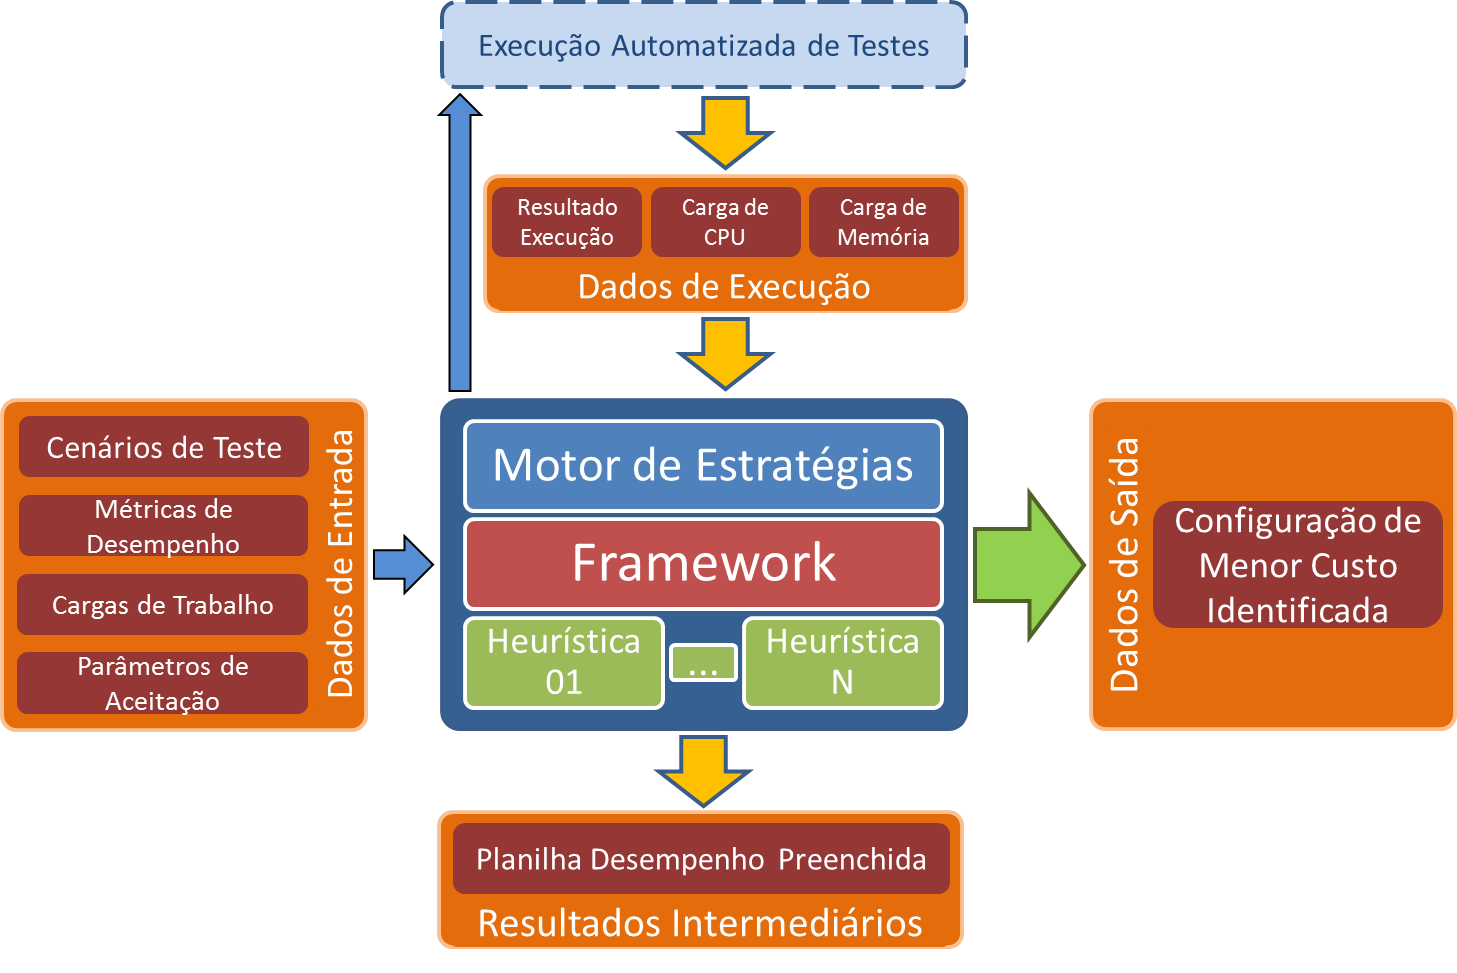
\includegraphics[scale=0.5]{img/arquiteturaAltoNivel}
  \end{center}
\end{figure}

As Heurísticas de Avaliação de Capacidade, conforme propostas neste trabalho, 
são implementações de estratégias que buscam encontrar, a partir do Resultado 
de uma Execução da Aplicação sob Teste sob uma Carga de Trabalho inicial em uma 
Configuração inicial, se existe uma Configuração mais barata que seja capaz de 
executar a mesma Carga de Trabalho.

O funcionamento de uma Heurística é totalmente baseado no caminhamento sobre o
Espaço de Implantação e sobre um a faixa de valores de Cargas de Trabalho. O 
tamanho de cada passo nesse caminho depende da lógica empregada pela Heurística 
e da avaliação do Resultado obtido. Cada passo dado pela Heuristica pode resultar 
em uma nova Execução dos testes ou em uma conclusão a respeito da capacidade da 
Configuração avaliada (e outras similares) de executar a Carga de Trabalho a um 
custo viável. Assim, a inteligência de uma Heurística está na forma como ela 
decide caminhar sobre o Espaço de Implantação e na faixa de Cargas de
Trabalho apresentados.

Apresentamos a seguir o modelo de como uma Heurística deve funcionar, a 
especificação do arcabouço de implementação construído nesse trabalho, começando
por descrever as operações que uma Heurística deve executar. 

\section{Operações Iniciais}
Para que uma Heurística de Avaliação de Capacidade seja compatível no âmbito deste trabalho, 
deve apresentar um conjunto mínimo de operações esperadas para que a lógica da
avaliação se complete e o resultado final obtido possa ser considerado válido e
comparável com os resultados obtidos por outras Heurísticas.

Além disso, as operações constituem a interface pela qual o controlador das 
sessões de avaliação pode configurar as Heurísticas e informar-lhe os dados 
necessários ao controle da sua execução.
 
Apresentamos esse conjunto mínimo de operações nas subseções a seguir, que 
representam o arcabouço necessário para a construção de uma Heurística de 
Avaliação de Capacidade.

\subsection{Selecionar Carga de Trabalho Inicial}
Este trabalho tem como premissa a necessidade de se identificar quais as 
Configurações mais baratas em um Provedor capazes de executar diversos níveis de
Cargas de Trabalho, tendo como objetivo a otimização de custos para a execução de
uma Aplicação so Teste.

Assim, pressupomos que exista uma faixa de valores para os níveis de Cargas de 
Trabalho a que a Aplicação é costumeiramente submetida e que seja de conhecimento
prévio dos responsáveis pela Aplicação. 

De posse dessa faixa de valores de Cargas de Trabalho, uma Heurística deve ser 
capaz de escolher, de acordo com sua estratégia de trabalho, um valor inicial de
Carga de Trabalho a ser imposta sobre a Aplicação. A Carga de Trabalho escolhida
deve ser retornada para o controlador da sessão, de forma que este possa coordenar
a Execução dos testes.
 
\subsection{Selecionar Configuração Inicial}
Analogamente, a fim de que as atividades da sessão de avaliação possam ter início,
é necessário que a Heurística de Avaliação de Capacidade usada selecione uma
Configuração inicial.

A escolha da Configuração inicial é feita a partir das Configurações disponíveis
no Espaço de Implantação previamente configurado pelo responsável pela avaliação.
A Heurística deverá avaliar o conjunto de configurações disponíveis quanto ao seu
preço, número de instâncias em cada, etc, de forma a escolher uma Configuração 
que considere mais adequada à sua estratégia para o início da sessão de avaliação.

\section{Operações de Controle}
Tendo em mãos uma Carga de Trabalho e uma Configuração iniciais, o controlador
da sessão de avaliação de capacidade pode ordenar uma Execução de testes, onde
serão coletados dados de desempenho relevantes para a Aplicação sob Teste.

Após a primeira Execução, um Resultado contendo os dados de desempenho colhidos 
é avaliado pelo controlador e, conforme sua decisão, novas Execuções podem se 
fazer necessárias. Neste caso, a Heurística deve ser novamente invocada, desta 
vez a selecionar uma nova Carga de Trabalho ou uma nova Configuração a partir do
Espaço de Implantação. Essa interação deve se repetir até que o controlador 
conclua os testes e dê por encerrada a sessão de avaliação.

Abaixo descrevemos as operações que a Heurística deve prover para que permita ao
controlador a correta operação dos testes e da sessão.

\subsection{Selecionar Nova Configuração}
Depois da cada execução de testes, o controlador estará de posse de um Resultado,
contendo os dados de desempenho da Aplicação executada sob a Carga de Trabalho e
a Configuração selecionadaa. A depender dos dados desse Resultado, o controlador
pode decidir executar novos testes em outra Configuração.

Para isso, a Heurística deve ser usada para selecionar a próxima Configuração a 
ser testada com a Aplicação. Com base no Resultado obtido pela Execução anterior,
a Heurística usará sua lógica de navegação para determinar a distância a ser 
caminhada no Espaço de Implantação em busca da nova Configuração.

A ordem de caminhamento é dada conforme a necessidade identificada pelo 
controlador, que vai definir se precisa de uma Configuração mais ou menos potente.
Porém, a Heurística é quem define, através de sua estratégia, qual será a próxima
Configuração usada.

Assim, a Heurística deve prover ao controlador duas operações para escolha da 
próxima Configuração: uma para Elevar o Nível de Configuração, ou seja, escolher
uma Configuração de capacidade superior, e outra para Reduzir o Nível de 
Configuração, isto é, escolher uma Configuração de capacidade inferior. Em ambos
os casos, a Heurística deverá usar como dado de entrada o Resultado da última 
Execução.

As Heurísticas são livres para usar os dados do Resultado como melhor lhe 
aprouverem, desde que a saída seja uma Configuração que ainda não tenha sido 
usada nos testes anteriores. 

\subsection{Selecionar Nova Carga de Trabalho}
De maneira similar à escolha de uma nova Configuração, o controlador pode usar
a Heurística para selecionar uma nova Carga de Trabalho, de acordo com o 
resultado com a última Execução.

As Heurísticas devem, então, prover operações que permitam a navegação pela
faixa de valores de Cargas de Trabalho estudada para a Aplicação sob Teste. 
Portanto, uma Heurística compatível deve fornecer duas operações de controle do
nível de Carga de Trabalho: uma operação para que seja reduzido e outra operação 
para que seja elevado o nível de Carga de Trabalho.

Aqui também as Heurísticas são livres para criarem suas próprias lógicas de 
avaliação dos dados do Resultado e, a partir daí, definirem qual o tamanho do
passo no caminhamento sobre a faixa de Cargas de Trabalho.
 
% ----------------------------------------------------------
